\section{Existing prototype}
\label{sec:existing_prototype}

At the beginning of the internship the existing code base (which was shortly described in chapter \ref{sec:goals}) was analyzed in order to understand how the ray casting application has been organized and implemented. The application is written in C++ using Microsoft Visual Studio 2010 and 2012. Beside the provided compilers from Microsoft, also Intel's C++ compiler is used during development to benefit from stronger optimization. The code makes heavy use of C++11 features and AVX SIMD instructions, thus limiting the application to rather up-to-date compilers (supporting C++11) and newer hardware (AVX is supported since Intel's Sandy Bridge and AMD's Bulldozer series). Furthermore, OpenMP is used as technology for high level parallelization, OpenGL for visualization and the MFC (Microsoft Foundation Class, a C++ wrapper of the Win32 API) for window and input management.
Considering the implemented algorithms, simply single ray casting (for subtraction volumes as shown in chapter \ref{sec:boolean_raycasting}) using the 3D DDA algorithm discussed in chapter \ref{sec:regular_grids} has been used in the beginning. However, the initial approach has then been replaced by a highly optimized and parallel packet ray caster using the slice traversing algorithm presented in chapter \ref{sec:packet_casting}. The single ray variant can still be found in the code but is not used anymore.

\subsection{Structure}

Figure \ref{fig:enlight_class_diagram} shows a simplified class diagram of the most relevant classes which are used in the existing ray casting implementation and have been dealt with when extending the existing infrastructure by the new OpenCL ray caster.

\begin{figure}
\centering
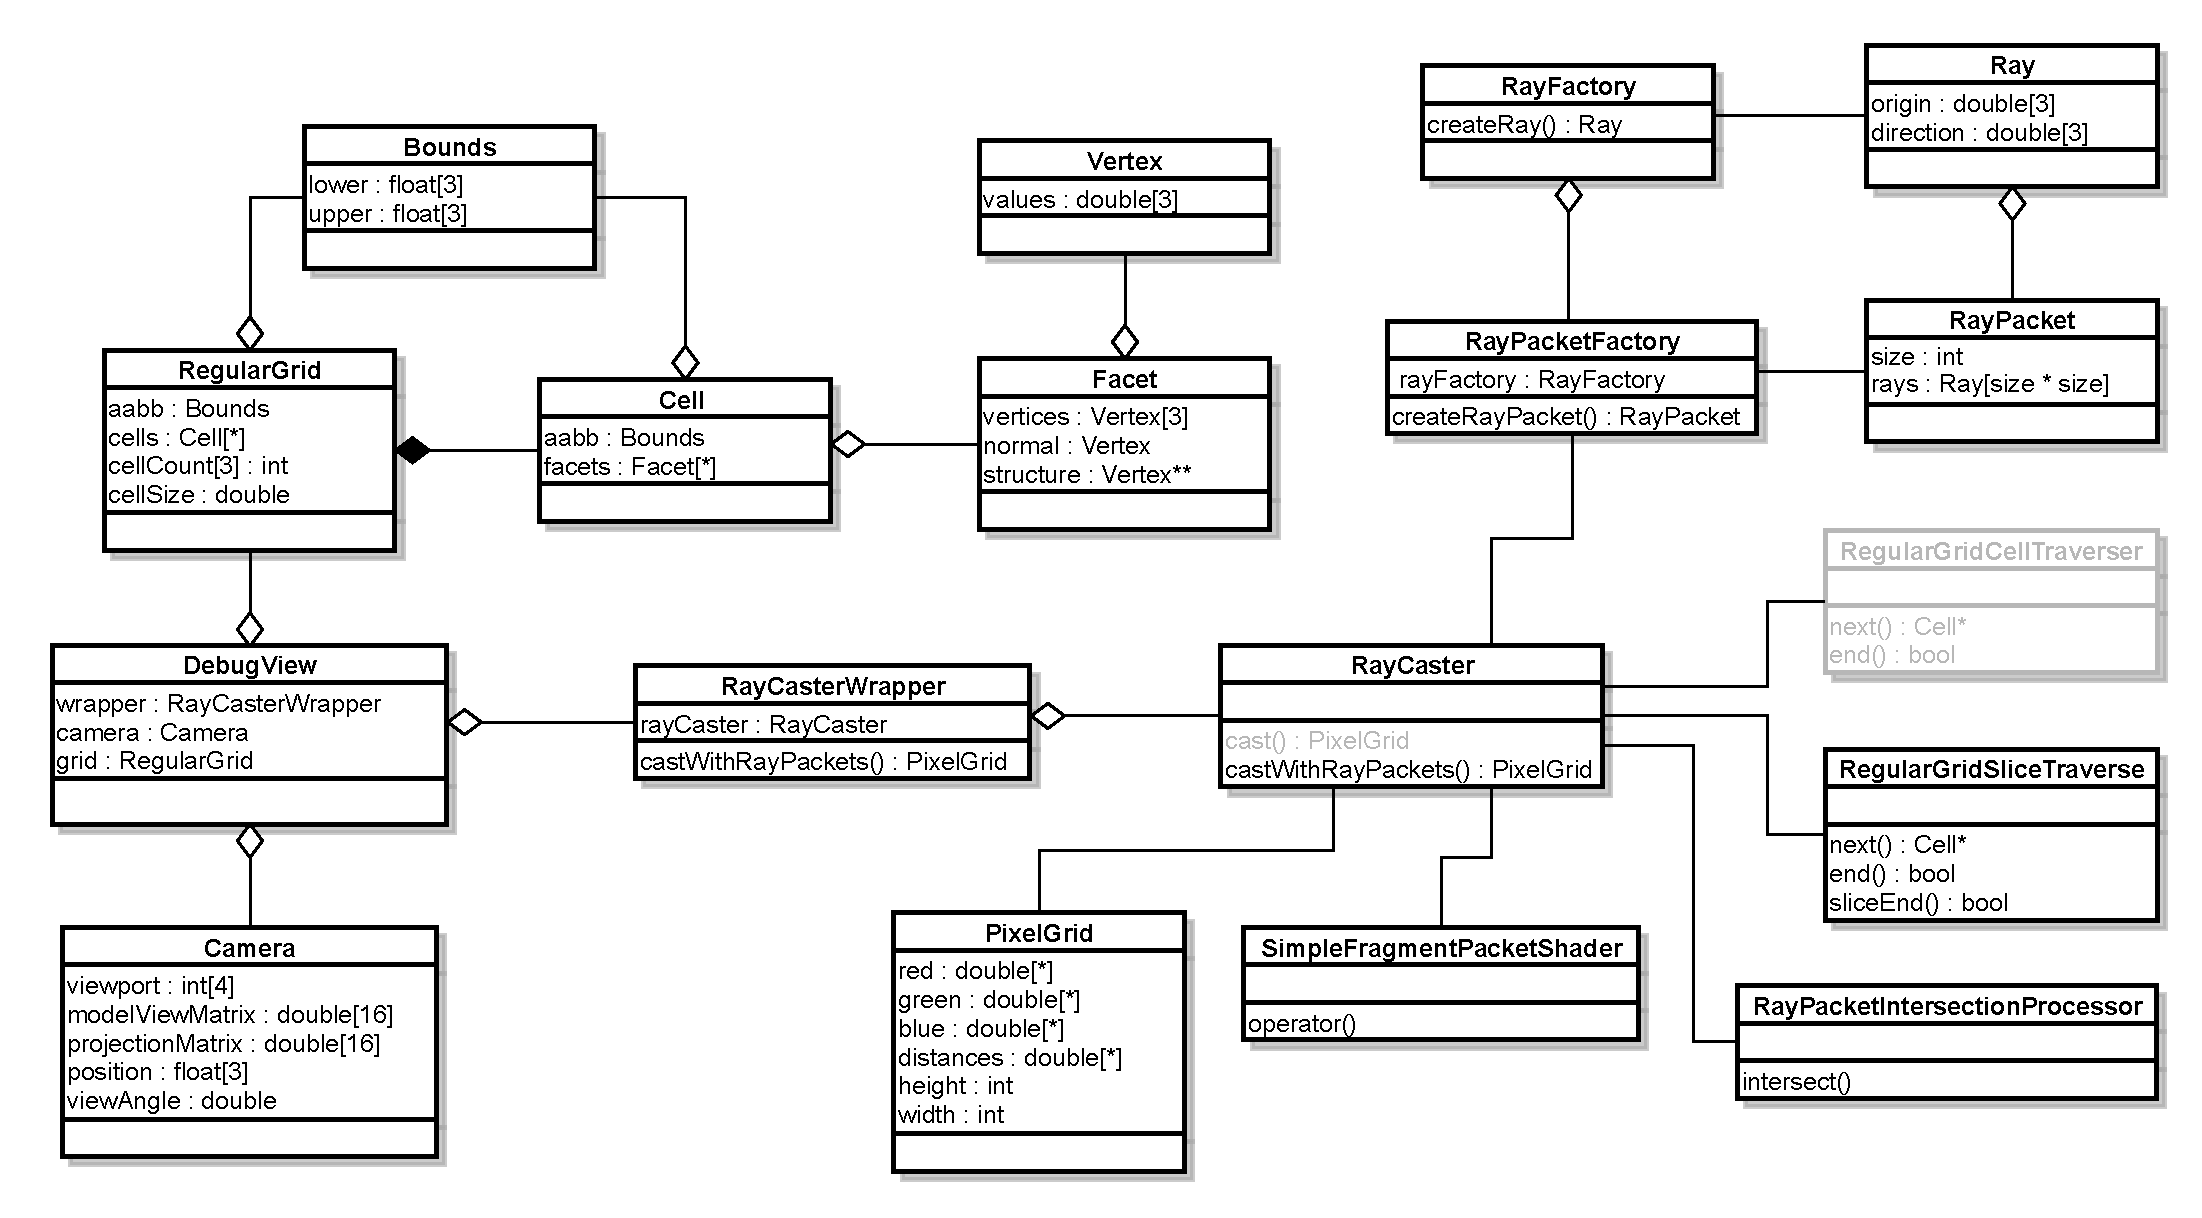
\includegraphics[width=\textwidth]{enlight_class_diagram}
\caption{Simplified class diagram of the most important classes involved in ray casting at the beginning of the internship.}
\label{fig:enlight_class_diagram}
\end{figure}

The central class containing most of the application logic is \lstinline!DebugView!. It inherits \lstinline!CWnd! from the MFC and is the main window of the application containing the OpenGL visualization. Beside all graphical user interactions like zooming and rotating using the cursor, also the console commands are parsed and processed within this class. It further contains an instance of \lstinline!Camera! which is updated according to user interaction. Also the regular grid holding all loaded meshes is stored by \lstinline!DebugView!. Finally, a wrapper class delegating to the ray casting implementation is also available (\lstinline!RayCasterWrapper!). When the application has been started, meshes can be loaded from the file system via corresponding console commands. The loaded meshes are processed by the classification algorithm and merged into the grid (covered in chapter \ref{sec:classification}). Ray casting can be triggered either by issuing a command on the console or altering a camera property via GUI input (zoom, rotation). In both cases, \lstinline!DebugView! eventually makes a call to \lstinline!castWithRayPackets()! from the ray casting implementation wrapper and passes a reference to the grid and current camera settings. The wrapper delegates this call to the corresponding method in \lstinline!RayCaster! where all the ray casting is done. At the beginning of every ray cast call, several camera values are retrieved and a \lstinline!RayPacketFactory! is created. This factory makes use of the older \lstinline!RayFactory! used for the initial single ray casting algorithm. Furthermore, an instance of \lstinline!PixelGrid! is created which will be later used to store the ray casting results and will be returned to the calling \lstinline!DebugView! class, where it is used to render the casted image. After this setup, the requested output image area (sized according to the width and height of the camera) is divided into a grid of square packets (adjustable size, currently eight) and iterated over by two nested for loops. The outer one of the loops iterates over the rows of the packets and is executed in parallel using an OpenMP directive. Within the inner loops, \lstinline!RayPacket!s are created using the corresponding factory. Each packet is then traversed through the grid using an instance of \lstinline!RegularGridSliceTraverser!. After the slice traverser has been initialized with the packet (which determines traversal axis and grid entry point), a while loop retrieves cells from the slice traverser using its \lstinline!next! method until \lstinline!end! returns true. On every slice end, the traversal may be early aborted if all rays of the packet have already hit. For each cell the slice traverser returns, the ray packet has to be intersected with the contained geometry. This is done using an instance of \lstinline!RayPacketIntersectionProcessor!. Here is most of the required CPU time consumed. Therefore the \lstinline!intersect! routine and all subroutines are highly optimized and consist to a high degree of AVX vector intrinsics. The intersection test for the packet is performed in parallel using SIMD after all triangles of the cell have been culled against the frustum defined by the corner rays of the packet (details will be discussed later in chapter \ref{sec:adapted_ray_casting}). For each intersection, the normal of the hit surface and the distance from the eye point are retrieved. The normal together with the initial ray direction of every ray of the packet is then used by the \lstinline!SimpleFragmentPacketShader! to calculate a color value for the ray. Currently, the dot product of both vectors is taken as a gray scale value to achieve simple shading. The distance of the intersection point to the eye point (camera position), from which the ray originated, is later translated into the normal distance of the intersection point to the image plane which corresponds to the depth value which would have been generated by OpenGL if the scene has been rendered traditionally. After all ray packets have been processed, the final \lstinline!PixelGrid! instance containing the color and depth values is returned back to \lstinline!DebugView! for display.

\subsection{Ray casting data structure}
\label{sec:data_structure}

The used data structure for holding the geometry and accelerating the ray casting algorithm is implemented by several classes. To start with, the \lstinline!RegularGrid! class is a simple container for cells. It also stores some meta information such as the grids bounding box, the number of cells in each dimension and the size of a cell. The cells are stored in a continuous array. Therefore, 3-dimensional cell coordinates have to be mapped to the linear memory region. \\
The cells themselves are simple bounding boxes containing references (pointers) to the triangles (called facets) contained within the cells. Although the bounding box is implicitly given by the cell's coordinates inside the grid and the grid's bounding box, the box is kept precalculated as it is often needed by the ray casting algorithm. \\
A \lstinline!Facet! itself then consists of its three vertices, a normal as well as the \lstinline!structure! pointer. The latter references the mesh (subtraction volume) this facet originates from. The importance of this value is later elaborated when discussing the details of the intersection routine in chapter \ref{sec:adapted_ray_casting}.

\subsection{Classification}
\label{sec:classification}

When a mesh is added to the grid, the triangles of the mesh have to be mapped to the cells of the grid. After the mapping is complete, the cells can be classified to one of three categories. Cells which are occupied with triangles of the mesh surface are surface cells. Cells inside the mesh are inside cells and contain no triangles. Cells outside the mesh are outside cells and also contain no triangles. For the ray casting algorithm, only surface cells are relevant. Figure \ref{fig:classification} illustrates the classification of a mesh.

\begin{figure}
\centering
\includegraphics[width=0.5\textwidth]{classification}
\caption{Principle of classifying cells of the grid according to the added mesh. Only surface cells are relevant for ray casting.}
\label{fig:classification}
\end{figure}

When a new mesh is added to the grid, the mesh is again classified and merged into the existing cell classification. Limiting the modifiability of the scene to only allowing the addition of further subtraction volumes makes the rules for merging a new mesh into the grid easy as seen in table \ref{tbl:classification_rules}.

\begin{table}[h]
\centering
\begin{tabular}{|c|c|c|c|c|}
\hline
\multicolumn{2}{|c|}{\multirow{2}{*}{merge}} & \multicolumn{3}{c|}{Cell class of subtraction volume} \\
\cline{3-5}
\multicolumn{2}{|c|}{} & outside & surface & inside \\
 \hline
\multirow{3}{*}{Cell class before} & outside & outside & outside & outside \\
\cline{2-5}
 & surface & surface & surface & outside \\
\cline{2-5}
 & inside & inside & surface & outside \\
\hline
\end{tabular}
\caption{Table of different merge scenarios and their outcome.}
\label{tbl:classification_rules}
\end{table}

Cells which are outside the added subtraction volume stay the same. Surface cells of the added volume become surface cells except they where outside cells before. And cells inside a subtraction volume always become outside cells. The result of merging a subtraction volume into the grid is visualized in figure \ref{fig:classification_sub}.

\begin{figure}
\centering
\includegraphics[width=0.5\textwidth]{classification_sub}
\caption{Classification result after adding a subtraction volume. }
\label{fig:classification_sub}
\end{figure}

As we can see, cells which where surface cells before and contained triangles have now become outside cells and are therefore no longer relevant for ray casting. As a result, the increase of triangles in the surface cells by adding new geometry has been compensated by exclusion of some surface cells. This reduction of potential triangles for intersection with an increasing number of subtraction volumes is vital, as it enables scalability, allowing even scenes with thousands of subtraction volumes to be ray casted efficiently. In fact, some scenes can even be casted faster with an increasing number of subtraction volumes as the number of relevant triangles (surface cells) decreases.

However, this kind of reduction has a significant consequence on the ray casting algorithm. As subtraction volumes are divided into grid cells and some of them discarded, the volumes are no longer water tight. This is a problem for entry/exit counting ray casting algorithms such as the one discussed in chapter \ref{sec:boolean_raycasting}. Therefore, an adapted version of this algorithm has to be developed, capable of handling open volumes. Chapter \ref{sec:adapted_ray_casting} discusses a method of getting around this problem.


\subsection{Adapted intersection algorithm}
\label{sec:adapted_ray_casting}

consequences of classification on raycasting algorithm

implicit geometry, water tightness? why no problem?

algorithm description of CPU caster
